\subsection{Sezione Utente}
\label{sec:sezUtente}

\par Una volta effettuato l'accesso al sistema, l'Utente visualizza una schermata con il nome e il simbolo di ChatSQL posizionati in alto a sinistra, mentre a destra si trovano il pulsante per le impostazioni e quello per il login. Sul lato sinistro, un menu consente di navigare tra le pagine dell'applicazione. A destra del menu, si trova la pagina principale, che rappresenta la chat del sistema e presenta un menu superiore. Al centro dello schermo, vengono visualizzati i messaggi inviati e/o ricevuti dall'Utente, mentre nella parte inferiore è possibile digitare nuovi messaggi.

\subsubsection{Interazione con la chat} \label{sec:interazione-chat}

\par Per interagire con la chat, è necessario inserire una richiesta nel box di testo situato in basso. È importante formulare interrogazioni che siano compatibili con il \glossario{dizionario dati} selezionato, in modo da ottenere un \glossario{prompt} corretto. I messaggi inviati dall'Utente vengono visualizzati a destra con uno sfondo azzurrino, mentre le risposte generate dal sistema vengono mostrate a sinistra con uno sfondo grigio scuro.

\begin{figure}[H]
  \centering
  %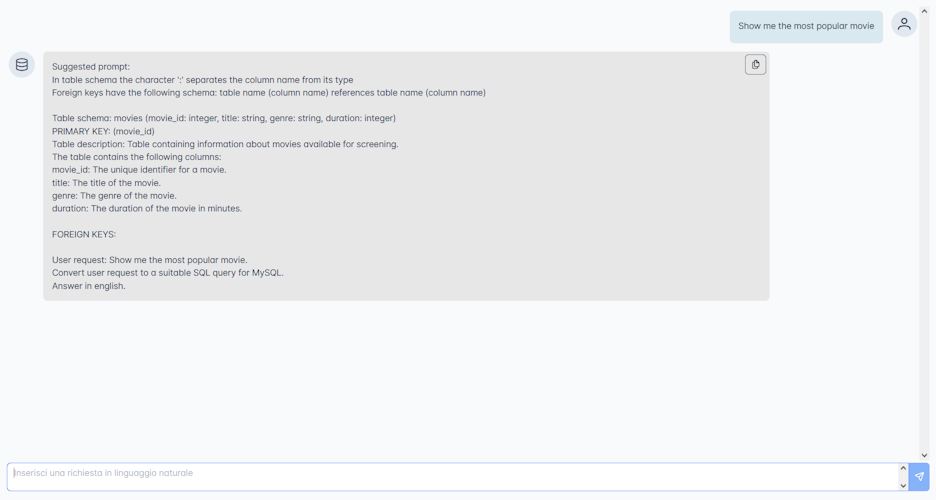
\includegraphics[width=\textwidth]{assets/chat_example.png}
  \caption{Esempio di interazione con la chat}
\end{figure}

\par Le richieste digitate dall'Utente possono essere inviate premendo il tasto Invio sulla tastiera o cliccando sul pulsante apposito accanto al box di testo. Questa azione rimuove il contenuto del campo di testo, permettendo all'Utente di inserire nuove richieste. Tuttavia, il messaggio inviato non viene rimosso e rimane visibile all'interno della chat.

\begin{figure}[H]
  \centering
  %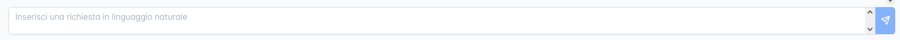
\includegraphics[width=\textwidth]{assets/text_box_arrow.png}
  \caption{Box di testo e pulsante di invio}
\end{figure}

\par C'è la possibilità che si verifichino errori durante l'elaborazione della richiesta e che il sistema non sia in grado di formulare il \glossario{prompt}. In tal caso, è consigliabile inserire una nuova richiesta, assicurandosi che sia coerente con il contenuto del \glossario{dizionario dati} scelto (\sezione{sec:info-dizionario}).

\begin{figure}[H]
  \centering
  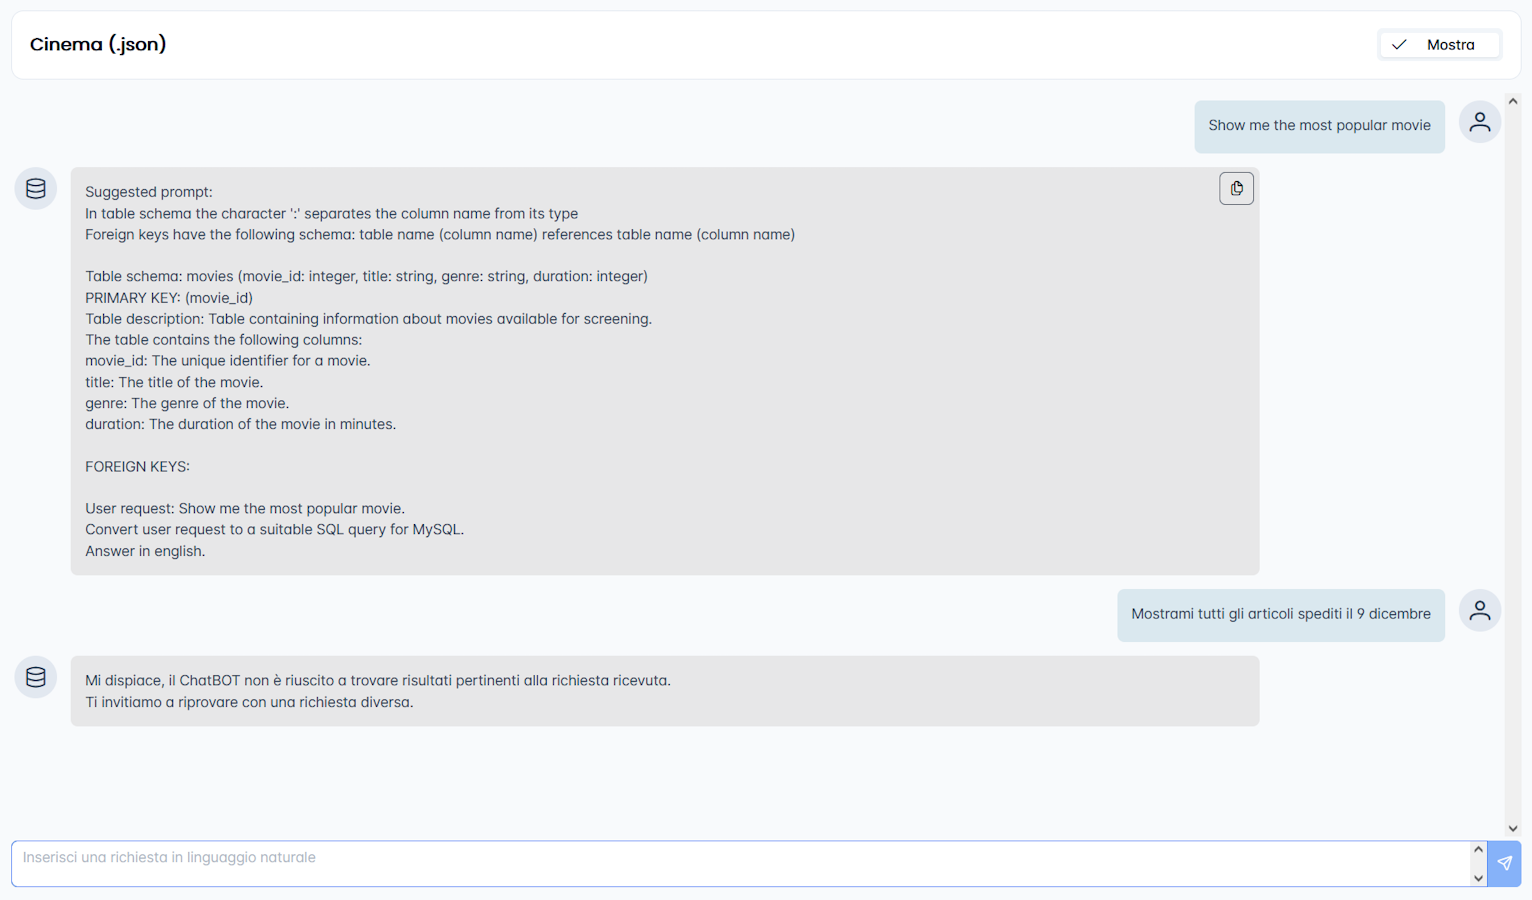
\includegraphics[width=\textwidth]{assets/es_chat_errore.png}
  \caption{Esempio di richiesta non idonea}
\end{figure}

\par Prima di inviare una richiesta al ChatBOT, l'Utente ha a disposizione le seguenti opzioni:
\begin{enumerate}
  \item Selezione/cambio dizionario dati;
  \item Accesso a informazioni aggiuntive sul dizionario dati scelto;
  \item Selezione/cambio DBMS;
  \item Selezione/cambio lingua.
\end{enumerate}

\subsubsubsection{Selezione/cambio dizionario dati}

\par Durante l'interazione con il sistema, è possibile cambiare il \glossario{dizionario dati} su cui si basano le richieste. Per selezionare un dizionario differente, l'Utente deve cliccare sul pulsante "Mostra" in alto a destra nella chat. Una volta aperto il menu, il dizionario dati attualmente in uso sarà elencato come la prima voce tra le quattro disponibili. Il dizionario dati può essere cambiato tramite un menu a tendina che mostra l'elenco dei dizionari.

\par Inoltre, è possibile cercare un dizionario scrivendo nella barra di ricerca che si apre cliccando sul menu a discesa. Una volta selezionato un dizionario, le richieste successive dovranno essere coerenti con il suo contenuto. Il pulsante "Nascondi" consente di chiudere il menu dopo aver completato la configurazione delle opzioni.

\begin{figure}[H]
  \centering
  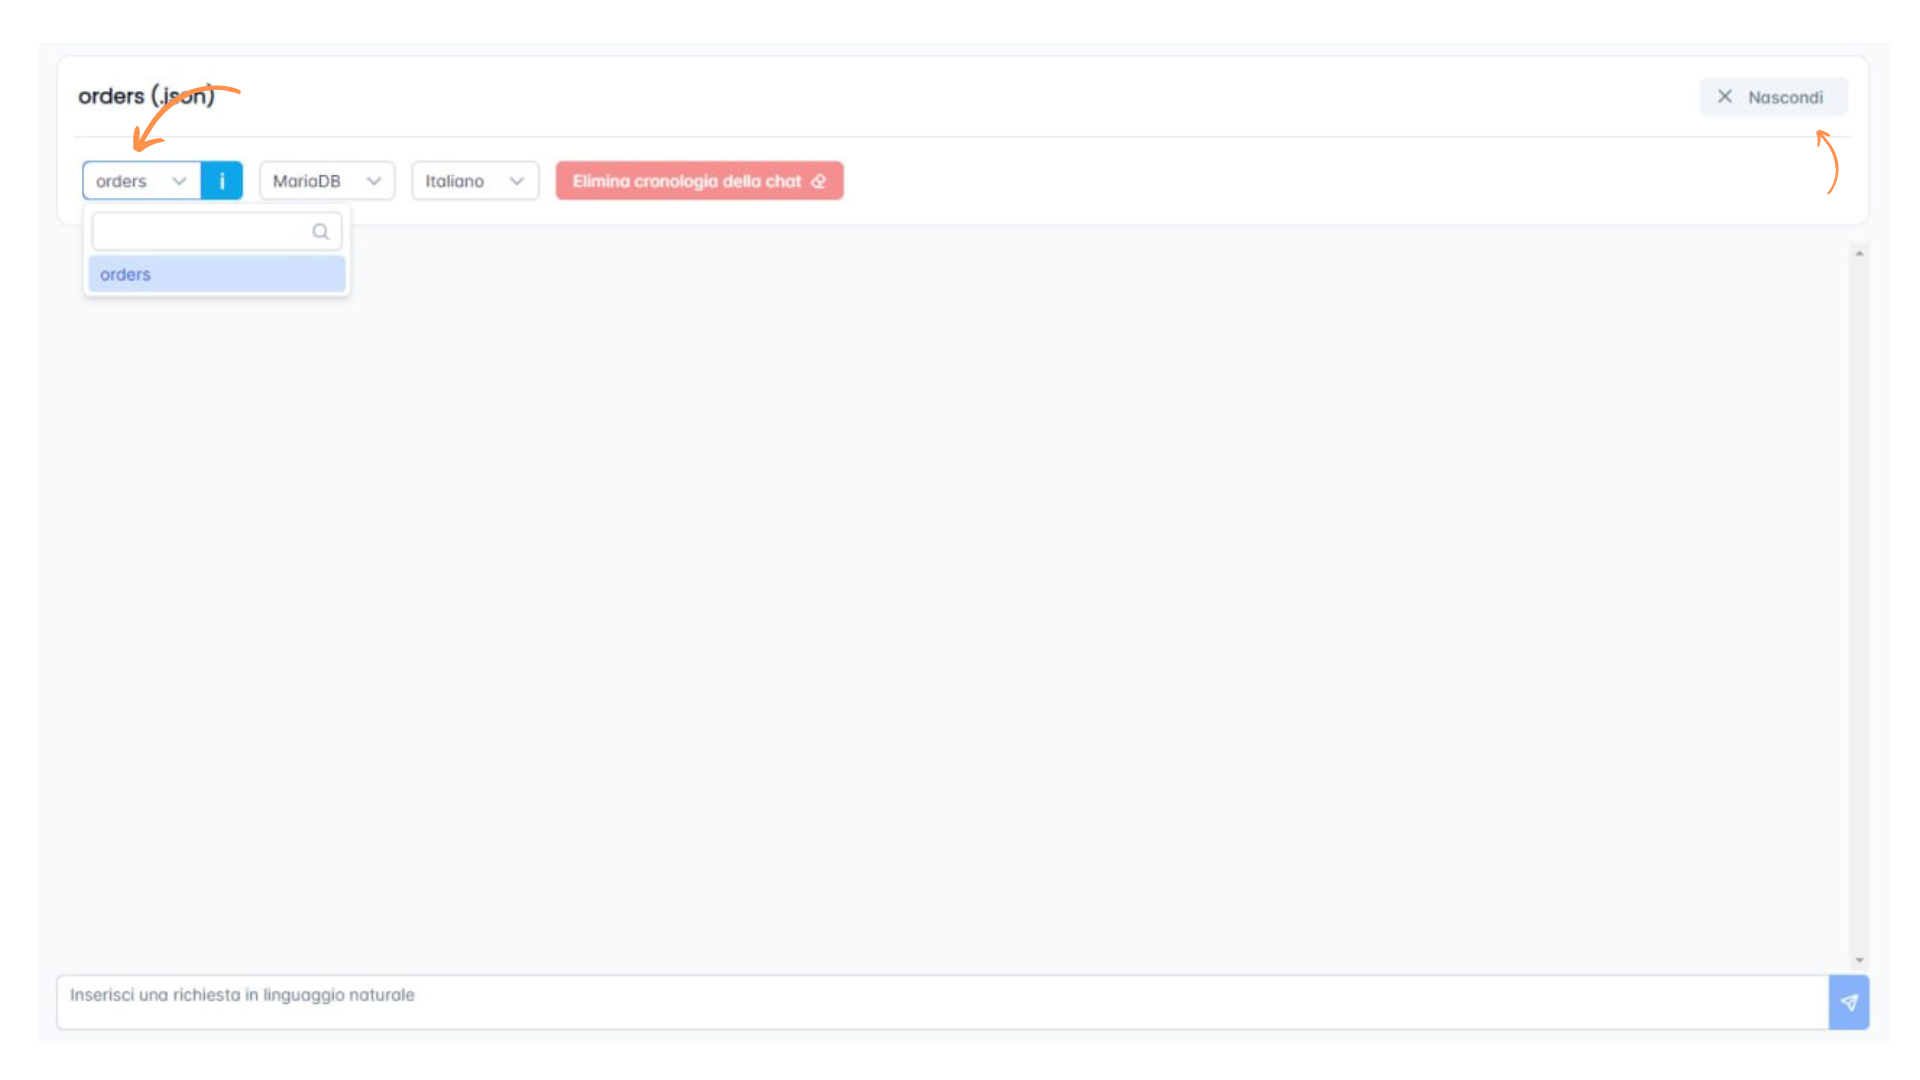
\includegraphics[width=1\textwidth]{assets/cambio_dizionariodati.png}
  \caption{Menu di selezione del dizionario dati}
\end{figure}

\subsubsubsection{Accesso a informazioni aggiuntive sul dizionario scelto} \label{sec:info-dizionario}

\par Accanto al menu a discesa, un pulsante con l'icona "i" consente di visualizzare un'anteprima del contenuto del dizionario selezionato. L'anteprima si sovrappone al contenuto della chat e mostra le seguenti informazioni:
\begin{itemize}
  \item Nome del dizionario;
  \item Descrizione del dizionario;
  \item Lista delle tabelle del \glossario{database} con le relative descrizioni.
\end{itemize}

\vspace{0.5\baselineskip}
\par La dimensione della scheda di anteprima può essere ingrandita o ridotta cliccando sul pulsante apposito all'interno della scheda stessa. In alternativa, l'anteprima può essere chiusa cliccando sulla "x" in alto a destra. Le informazioni contenute nella scheda di anteprima possono essere utilizzate come spunto per formulare una richiesta idonea. Una volta inviato un messaggio, l'anteprima verrà automaticamente chiusa.

\begin{figure}[H]
  \centering
  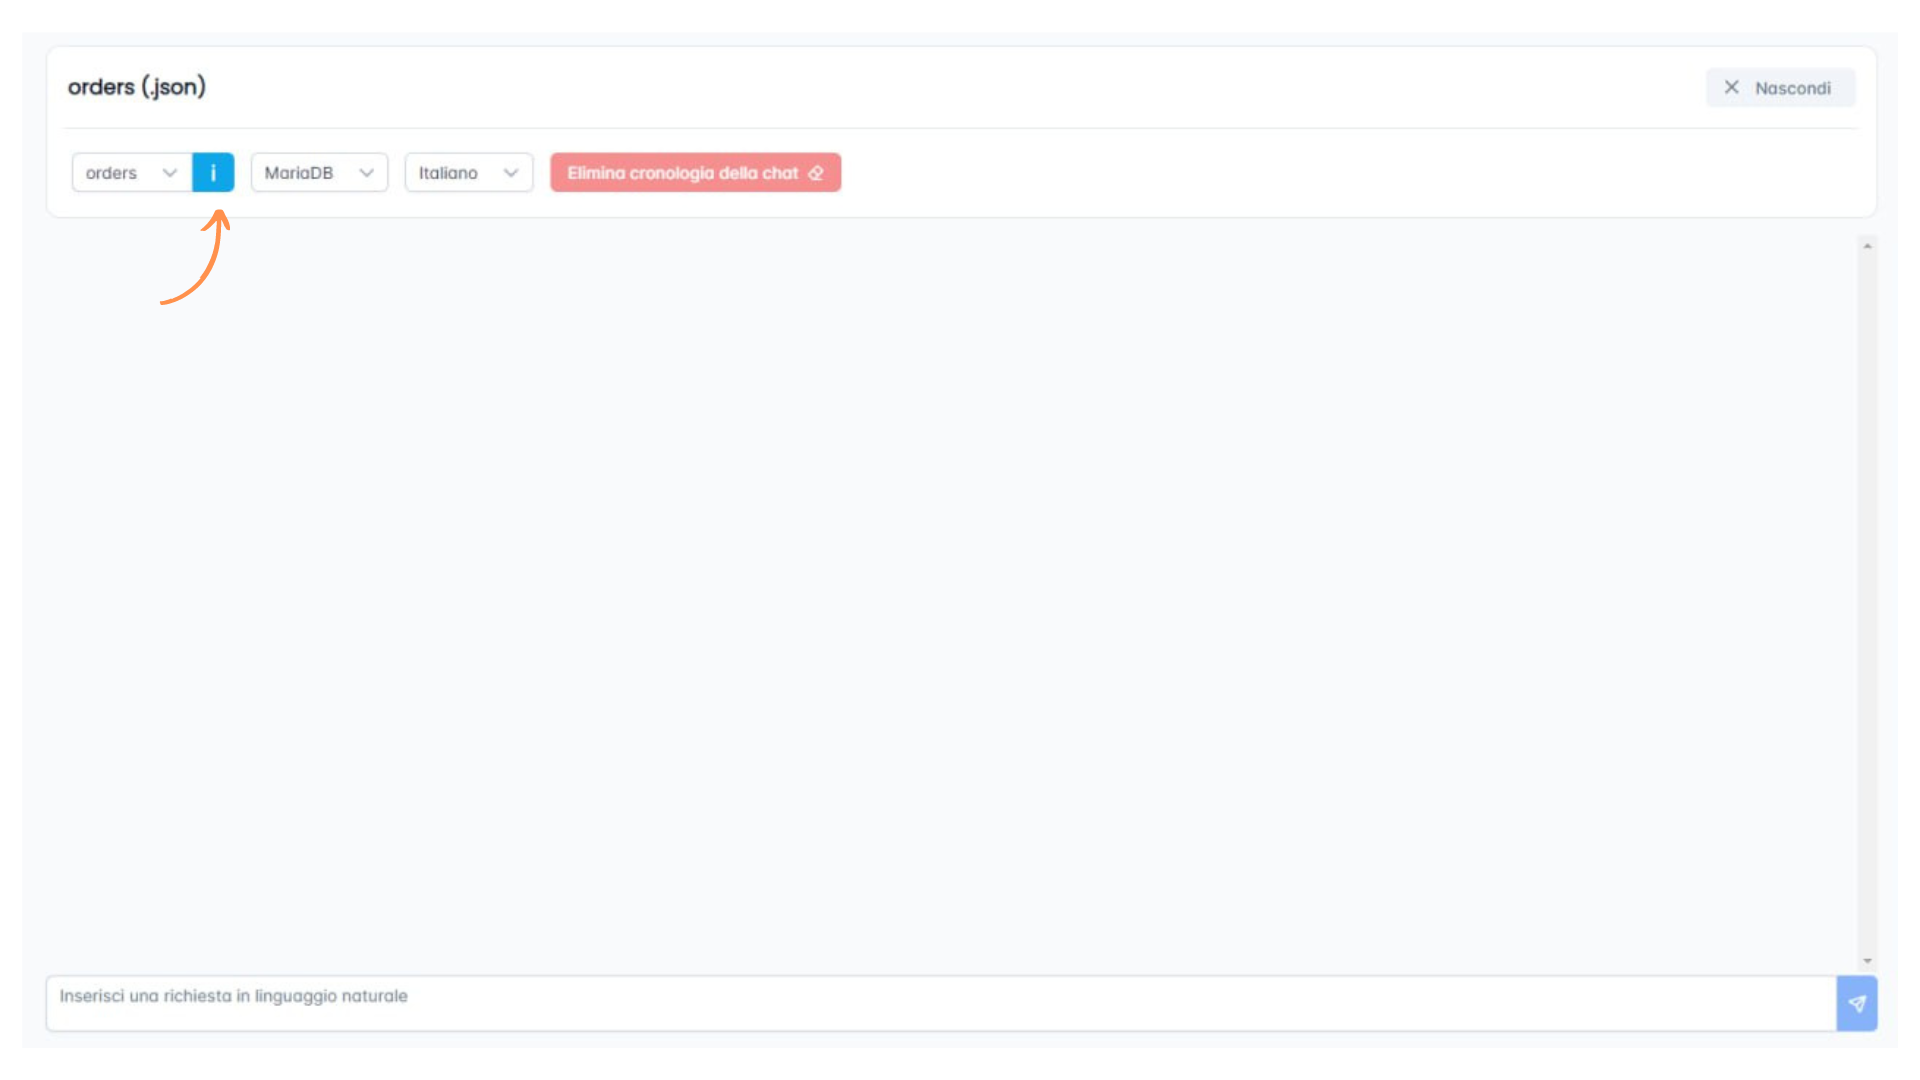
\includegraphics[width=1\textwidth]{assets/info_dizionario.png}
  \caption{Informazioni aggiuntive sul dizionario scelto}
\end{figure}

\subsubsubsection{Selezione/cambio DBMS}

\par Il sistema consente all'Utente di selezionare un \glossario{DBMS} tramite un menu a discesa analogo a quello sopra indicato. La selezione del DBMS segue le stesse modalità della scelta del \glossario{dizionario dati}. I DBMS supportati dal sistema sono i seguenti:
\begin{itemize}
  \item PostgreSQL;
  \item MariaDB (DBMS predefinito);
  \item Microsoft SQL Server;
  \item Oracle DB;
  \item SQLite.
\end{itemize}

\vspace{0.5\baselineskip}
\par La scelta del DBMS è cruciale per la generazione del \glossario{prompt}. Anche se \glossario{SQL} è un linguaggio standard, ci sono variazioni specifiche per ciascun DBMS. Per assicurarsi che gli \glossario{LLM} generino query corrette, è fondamentale che il prompt specifichi anche il DBMS di destinazione.

\begin{figure}[H]
  \centering
  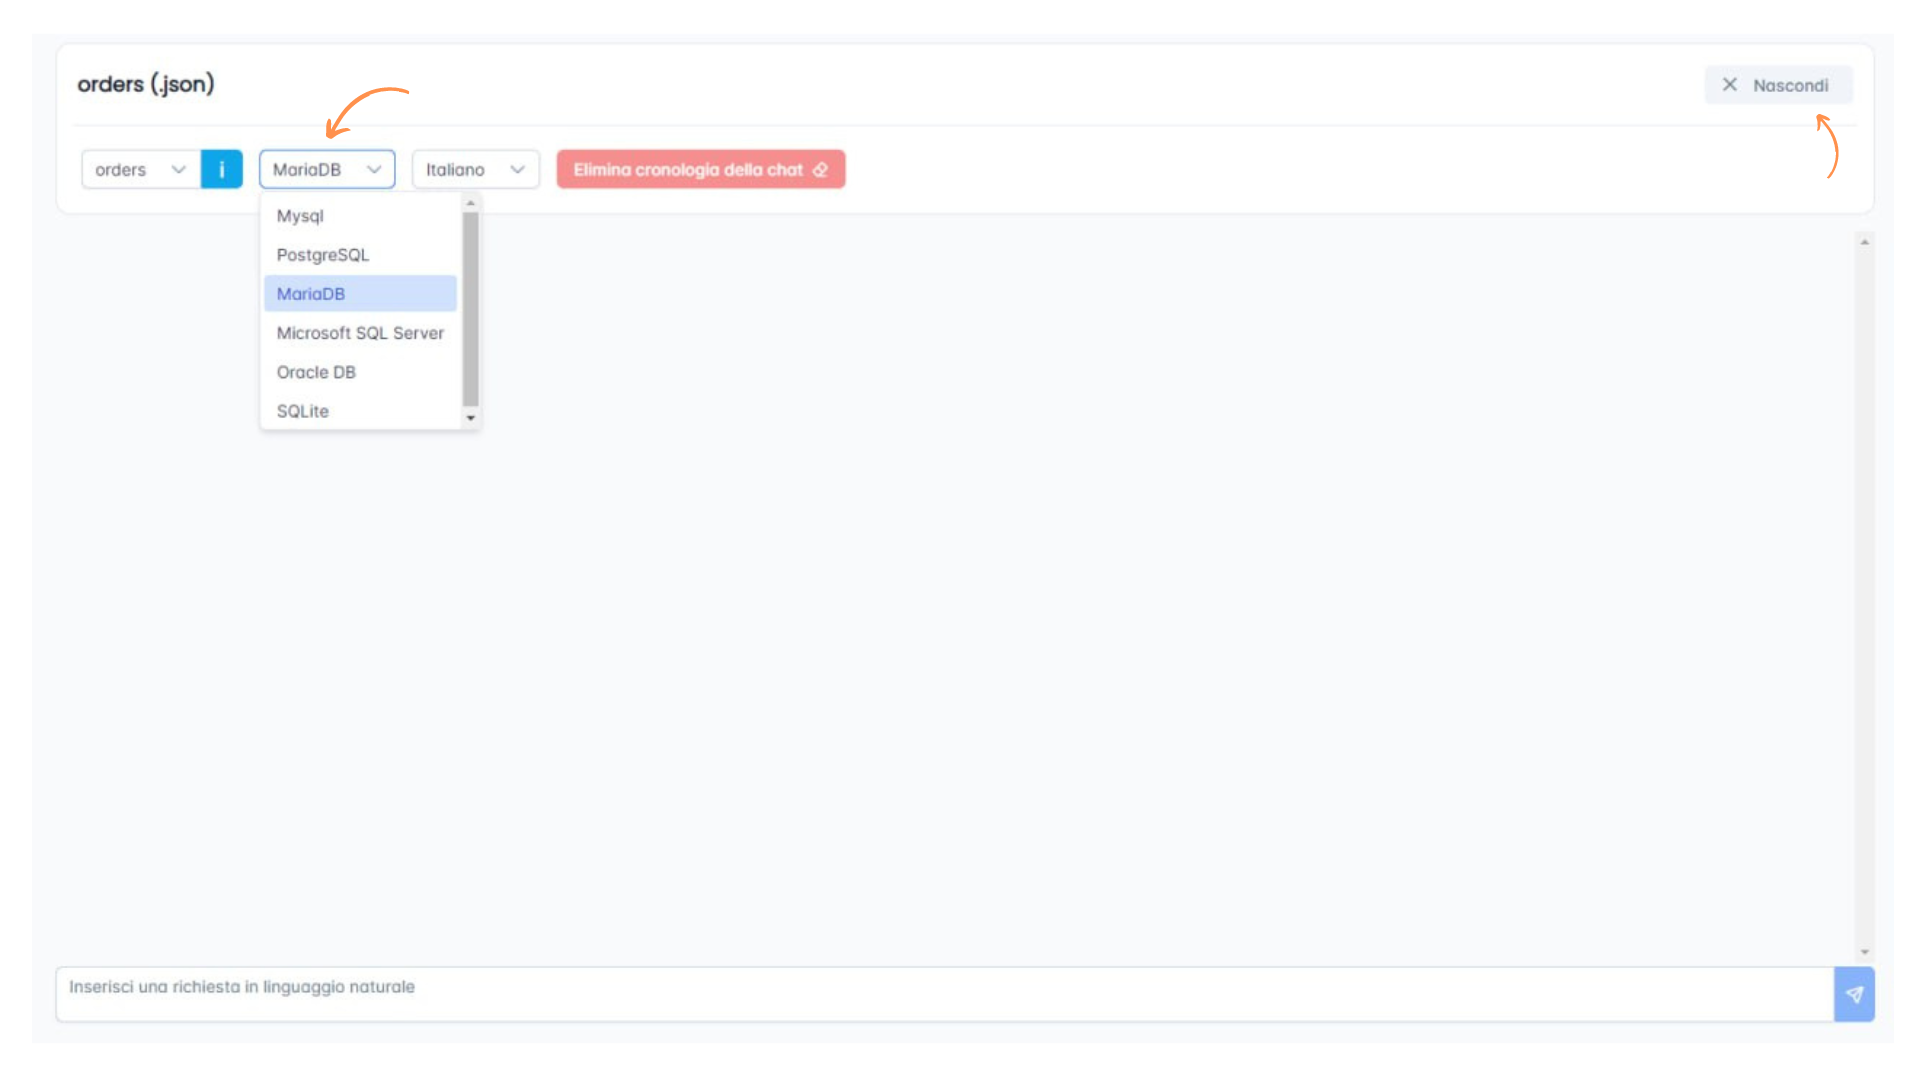
\includegraphics[width=1\textwidth]{assets/cambio_dbms.png}
  \caption{Menu di selezione del DBMS}
\end{figure}

\subsubsubsection{Selezione/cambio lingua} \label{sec:lingua-chat}

\par La selezione della lingua avviene anch'essa tramite un menu a discesa, in modo analogo alla scelta di dizionari e DBMS. Le lingue supportate dal sistema sono le seguenti:
\begin{itemize}
  \item Inglese (lingua predefinita);
  \item Italiano;
  \item Francese;
  \item Spagnolo;
  \item Tedesco.
\end{itemize}

\vspace{0.5\baselineskip}
\par La lingua selezionata viene inclusa nel \glossario{prompt} finale, in modo che la risposta dell'\glossario{LLM} utilizzato per generare la query \glossario{SQL} sia conforme alla lingua desiderata. Nonostante il prompt sia in inglese, l'inserimento della lingua consente agli LLM di adattare la propria risposta alla lingua scelta dall'Utente.

\begin{figure}[H]
  \centering
  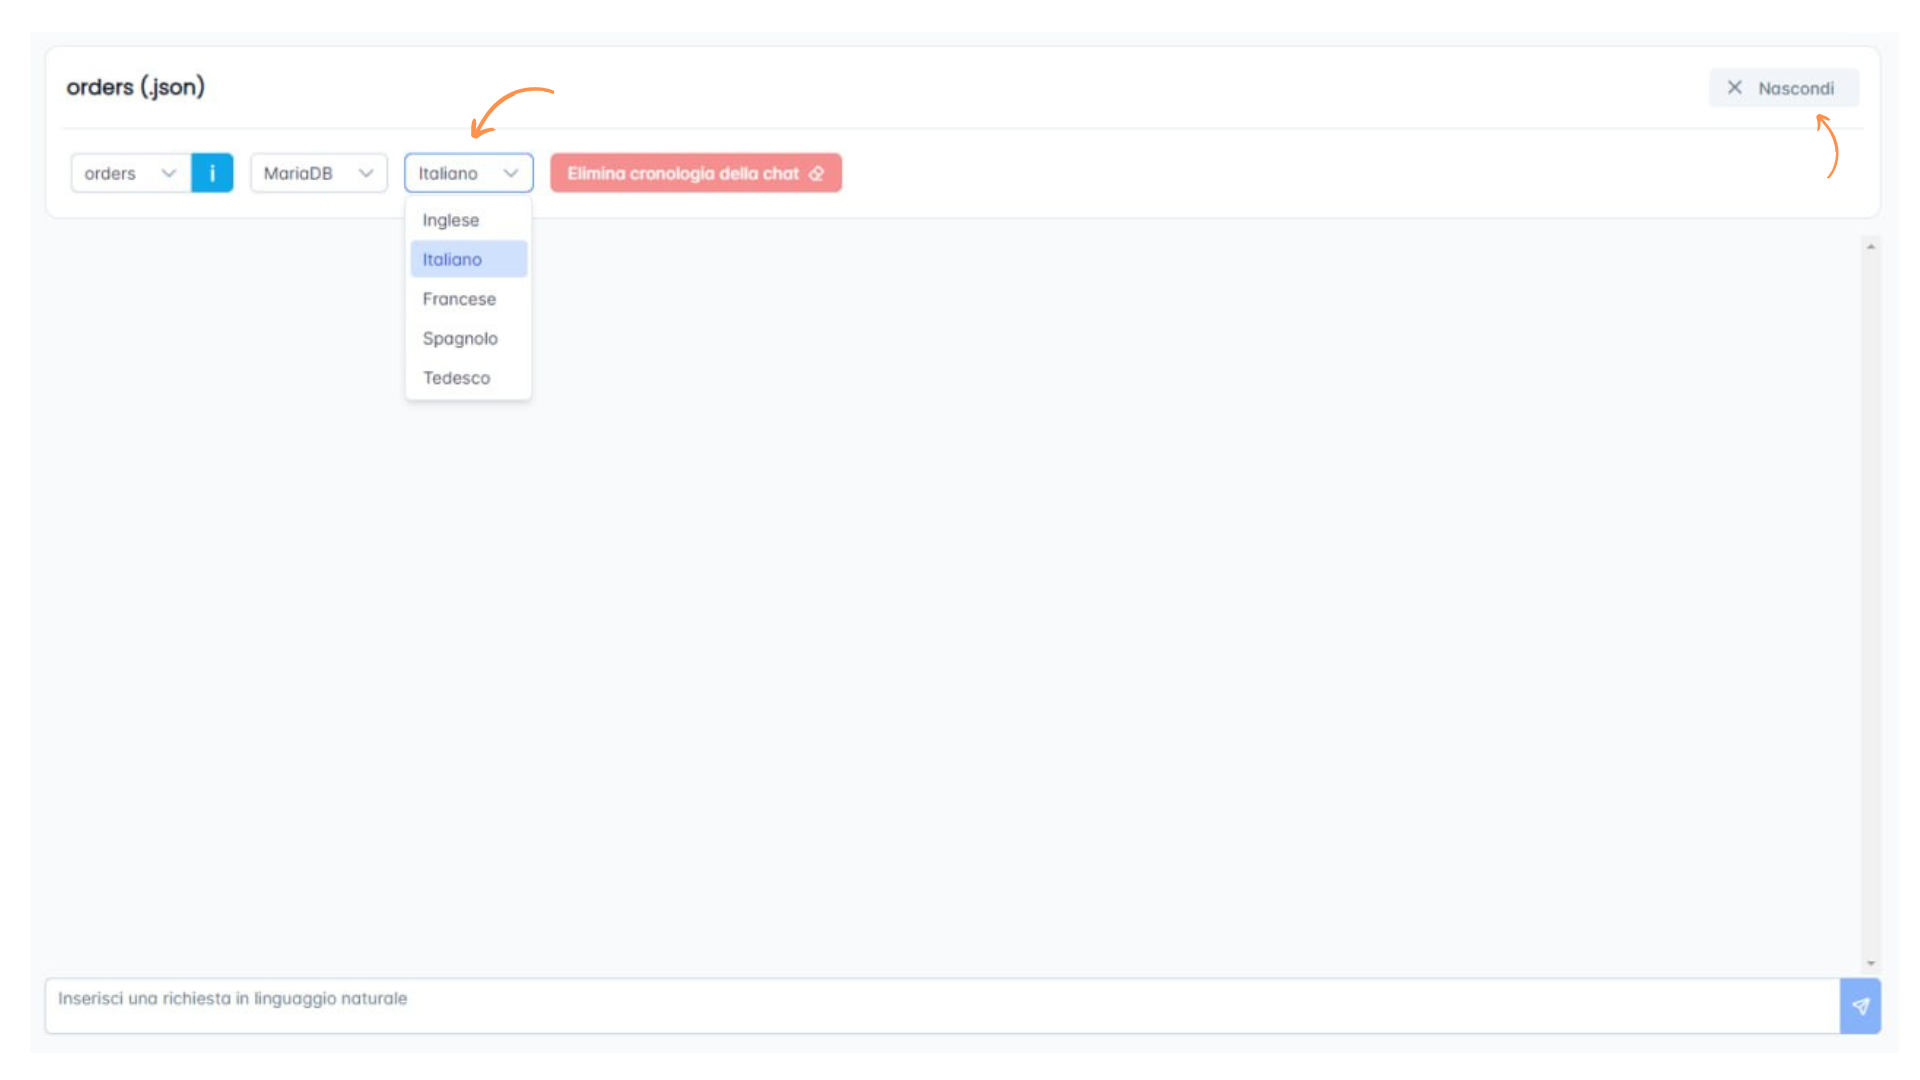
\includegraphics[width=1\textwidth]{assets/cambio_lingua.png}
  \caption{Menu di selezione della lingua}
\end{figure}

\par Una volta inviato il messaggio, l'Utente ha a disposizione le seguenti opzioni:
\begin{enumerate}
  \item Eliminazione della chat;
  \item Copia del prompt;
  \item Scorrimento automatico della chat.
\end{enumerate}

\subsubsubsection{Eliminazione della chat}

\par Dopo una conversazione prolungata con il ChatBOT, l'Utente potrebbe desiderare di eliminare le richieste e i prompt generati fino a quel momento, cancellando la cronologia della chat. Questa operazione può essere effettuata cliccando sul pulsante "Elimina cronologia della chat", che si trova all'interno del menu di selezione dei dizionari. Una volta cancellati, i messaggi verranno rimossi permanentemente dal sistema.

\begin{figure}[H]
  \centering
  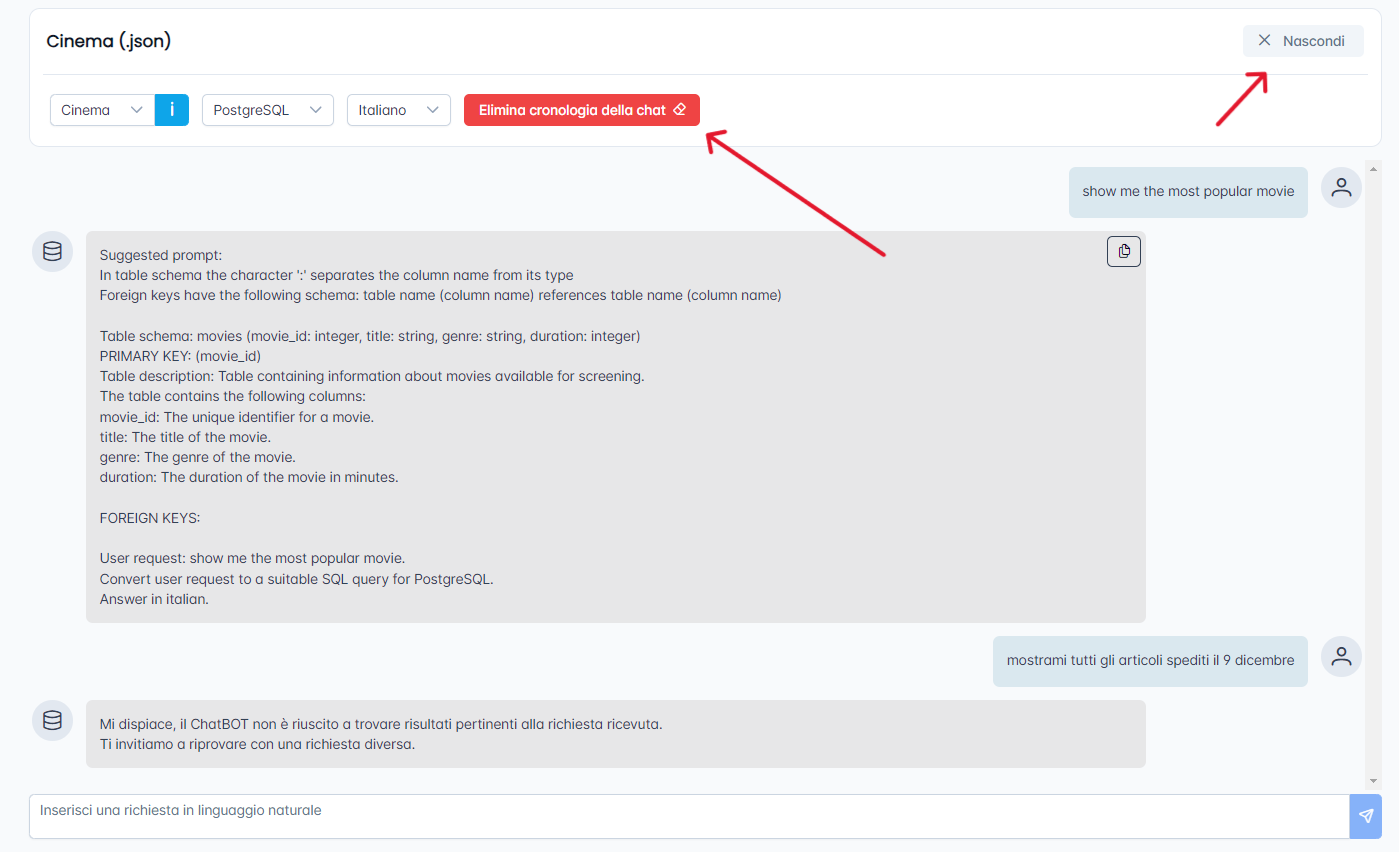
\includegraphics[width=1\textwidth]{assets/elimina_chat.png}
  \caption{Eliminazione della cronologia della chat}
\end{figure}

\subsubsubsection{Copia del prompt}

\par L'Utente può copiare il \glossario{prompt} generato dal sistema cliccando sull'icona di clipboard in alto a destra. Il testo copiato negli Appunti può essere incollato successivamente in altri applicativi e/o in un sistema di intelligenza artificiale come ChatGPT.

\begin{figure}[H]
  \centering
  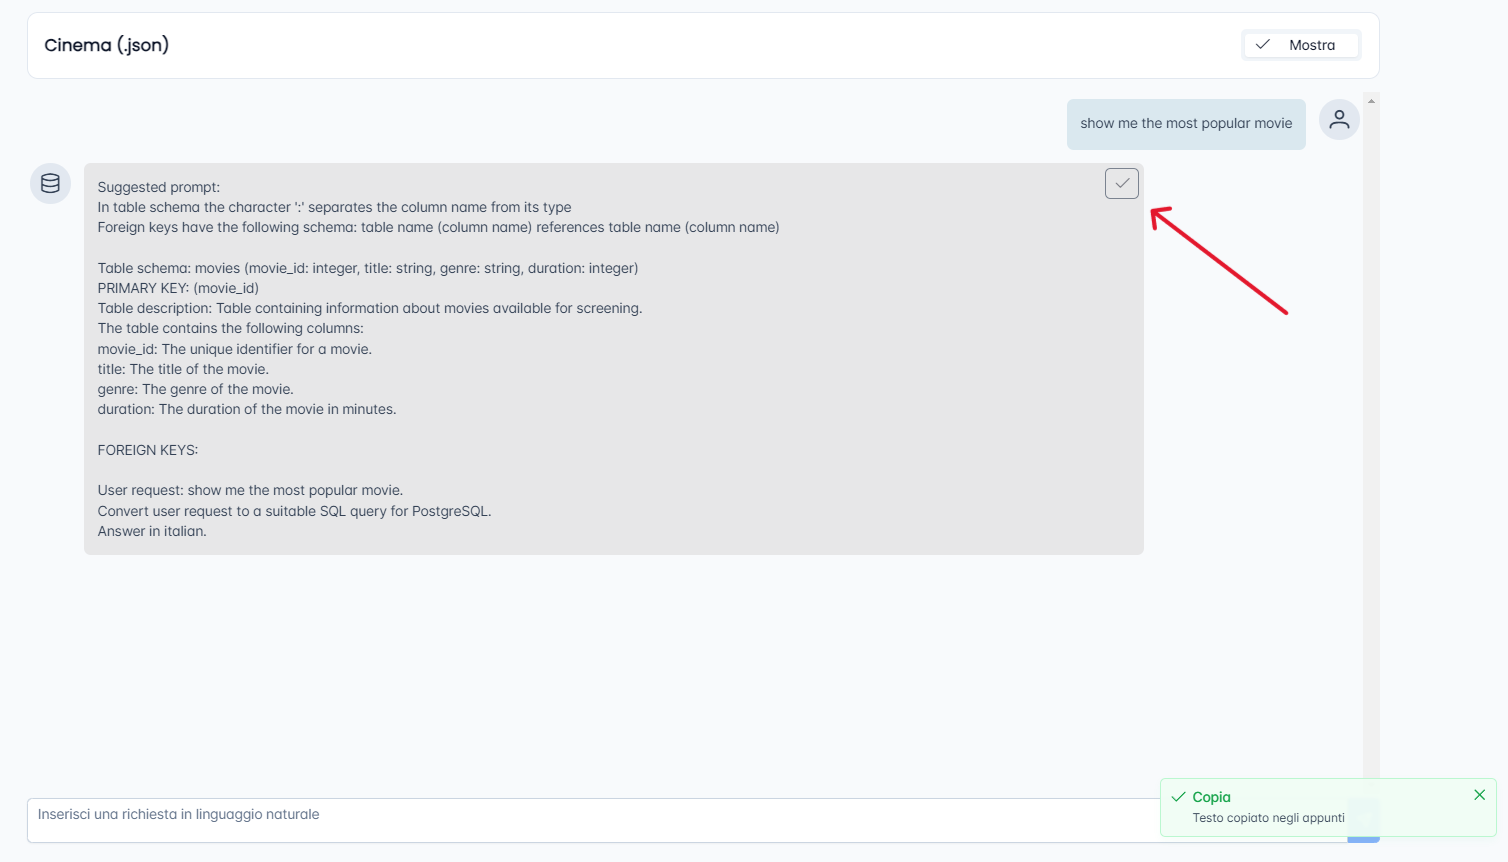
\includegraphics[width=1\textwidth]{assets/copia.png}
  \caption{Copia del prompt}
\end{figure}

\subsubsubsection{Scorrimento automatico della chat} \label{sec:scorrimento-chat}

\par Quando l'Utente scorre i messaggi, il sistema mostra un pulsante per tornare in fondo alla chat. Cliccando su di esso, l'Utente può visualizzare l'ultimo messaggio inviato o ricevuto. Al caricamento della pagina, se sono presenti messaggi salvati, il sistema scorre automaticamente fino alla fine della chat.